\documentclass{beamer}
\special{landscape}

%\usetheme{Berlin}
\usetheme{Warsaw}

%\usecolortheme{seahorse}
%\usefonttheme[onlysmall]{structurebold}

\setbeamertemplate{headline}[split]
\setbeamertemplate{footline}[default]
\setbeamertemplate{footline}[miniframes theme]
%\logo{\includegraphics[scale=0.25]{lifia_logo.png}}

\mode<presentation>
\usepackage[spanish]{babel}
\usepackage{beamerthemesplit}
\usepackage[utf8]{inputenc}
\usepackage{color}      % use if color is used in text


% Comandos en modo Verbatim
%\usepackage{fancyvrb}


\title{Practica 3 - Parte 4 - Anexo CDMA}
%\author{Juan Antonio Zubimendi\\azubimendi@lifia.info.unlp.edu.ar}

%\institute{LINSE}
%\date{24/04/2008}

\AtBeginSection[]

\begin{document}

\begin{frame}
%\frametitle{Presentación}
\titlepage
\end{frame}

\section{Controlador de DMA}
\subsection{Introducción}
\begin{frame}
\frametitle{Controlador de DMA}
%\begin{block}{Slot Accounting System}
\begin{itemize}
  \item ¿Que es DMA?
  \item Nos permite realizar transferencias de datos de 8 bits memoria-memoria, memoria-periférico o periférico-memoria.
  \item Por ser una transferencia DMA la CPU no interviene, pero si debe cederle el bus al CDMA.
  \item En el simulador hay que utilizar la Configuración 3 (c3).
\end{itemize}
\end{frame}

\subsection{Caracteristicas}
\begin{frame}
\frametitle{Caracteristicas}
%\begin{block}{Slot Accounting System}
\begin{itemize}
  \item El simulador posee un solo canal DMA
  \item Puede realizar transferencias en dos modos diferentes:
\begin{itemize}
  \item Modo Bloque: Se enviará el bloque completo una vez iniciada la transferencia
  \item Modo Bajo demanda: del periferico al que se encuentre conectado
\end{itemize}
  \item Cuando el CDMA termina de realizar la transferencia genera una interrupción.
  \item El CDMA está conectado a la línea de interrupción 3 del PIC.
\end{itemize}
\end{frame}

\subsection{Conexión}
\begin{frame}
\frametitle{Conexión}
\includegraphics[scale=0.45]{conf3.png}
\end{frame}

\subsection{Registros}
\begin{frame}
\frametitle{Registros}
  El controlador de DMA posee los siguientes registros
\begin{itemize}
 \item \emph{CTRL}: Un registro de control que nos permite configurar el funcionamiento del CDMA
 \item \emph{RF}: Registro de direcciones fuente.
  \begin{itemize}
    \item En transferencias memoria-periferico o periferico-memoria, indica la memoria de donde leer o a donde escribir.
    \item En transferencias memoria-memoria, es la posición de memoria de los datos a copiar.
  \end{itemize}
 
 \item \emph{RD}: Registro de direcciones destino. 
  \begin{itemize}
    \item Solo tiene sentido si es memoria-memoria.
  \end{itemize}
 \item \emph{CONT}: Registro Contador. Indica el número de bytes a transferir
 \item \emph{ARRANQUE}: Registro de Arranque. Accediendo a este registro, se inicia la transferencia.
\end{itemize}
\end{frame}

\begin{frame}
\frametitle{Registro de Control}
  \begin{center}
      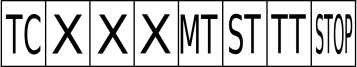
\includegraphics[scale=0.45]{cdma-ctrl.png}
  \end{center}

  \begin{itemize}
   \item El formato del registro \emph{CTRL} depende si lo estamos leyendo o escribiendo.
  \end{itemize}
  \begin{itemize}
     \item En lectura
     \begin{itemize}
        \item \emph{STOP}:
	  \begin{itemize}
	      \item 0: Transferencia en Curso
	      \item 1: Transferencia detenida por la CPU
	  \end{itemize}
        \item \emph{TC}:
	  \begin{itemize}
	      \item 0: Transferencia no finalizada
	      \item 1: Transferencia ya finalizada
	  \end{itemize}
     \end{itemize}
  \end{itemize}
\end{frame}


\begin{frame}
\frametitle{Registro de Control}
  \begin{itemize}
     \item En escritura
     \begin{itemize}
        \item \emph{STOP}:
	  \begin{itemize}
	      \item 0: No tiene sentido
	      \item 1: Detener momentaneamente la transferencia en curso
	  \end{itemize}
        \item \emph{TT}: Tipo de Transferencia
	  \begin{itemize}
	      \item 0: Transferencia Periferico-Memoria o Memoria-Periferico
	      \item 1: Transferencia Memoria-Memoria
	  \end{itemize}
        \item \emph{ST}: Sentido de la Transferencia (solo TT=0)
	  \begin{itemize}
	      \item 0: Sentido Periférico-Memoria
	      \item 1: Sentido Memoria-Periferico
	  \end{itemize}
        \item \emph{MT}: Modo de Transferencia
	  \begin{itemize}
	      \item 0: Por demanda
	      \item 1: Por Bloques
	  \end{itemize}

     \end{itemize}
  \end{itemize}
\end{frame}

\begin{frame}
\frametitle{Direccionamiento}
  \begin{itemize}
     \item Los registros se ubican a partir de la dirección 50h
     \begin{itemize}
        \item \emph{RF}: es de 16 bits 
	\begin{itemize}
	  \item \emph{RFL}: 050h - parte baja de \emph{RF}
	  \item \emph{RFH}: 051h - parte alta de \emph{RF}
	\end{itemize}
        \item \emph{CONT}: es de 16 bits 
	\begin{itemize}
	  \item \emph{CONTL}: 052h - parte baja de \emph{CONT}
	  \item \emph{CONTH}: 053h - parte alta de \emph{CONT}
	\end{itemize}
        \item \emph{RD}: es de 16 bits 
	\begin{itemize}
	  \item \emph{RDL}: 054h - parte baja de \emph{RD}
	  \item \emph{RDH}: 055h - parte alta de \emph{RD}
	\end{itemize}
        \item \emph{CTRL}: 056h
        \item \emph{ARRANQUE}: 057h
     \end{itemize}
  \end{itemize}
 
\end{frame}

\subsection{Uso}
\begin{frame}
\frametitle{¿Cómo lo usamos?}
  \begin{itemize}
     \item Demasiadas opciones, demasiadas configuraciones...
     \item Veamos para que lo vamos a utilizar en el simulador...
     \begin{itemize}
	\item Para copiar una parte de la memoria a otra posición
        \item Para mandar caracteres a la impresora a través del HAND-SHAKE
     \end{itemize}
  \end{itemize}
\end{frame}


\begin{frame}
\frametitle{Memoria-Memoria}
  \begin{itemize}
     \item Configuramos el registro de Control
     \begin{itemize}
	\item Tipo Transferencia: Memoria-Memoria
        \item Modo Transferencia: Bloques
     \end{itemize}
     \item Configuramos el registro \emph{RF} con la posición origen de la memoria
     \item Configuramos el registro \emph{RD} con la posición destino de la memoria
     \item Configuramos el registro \emph{CANT} con la cantidad de bytes a transferir
     \item Configuramos el PIC y una manejador de interrupción para saber cuando la transferencia terminó.
     \item Acceder al registro \emph{ARRANQUE} para iniciar la transferencia
  \end{itemize}
\end{frame}

\begin{frame}
\frametitle{Ejemplo Memoria-Memoria}
Veamos el ejercicio 1 del anexo de la práctica 3
\end{frame}

\begin{frame}
\frametitle{Memoria-Periferico}
  \begin{itemize}
     \item Configuramos el registro de Control
     \begin{itemize}
	\item Tipo Transferencia: Memoria-Periferico
        \item Sentido Transferencia: Memoria-Periferico
        \item Modo Transferencia: bajo demanda
     \end{itemize}
     \item Configuramos el registro \emph{RF} con la posición origen de la memoria
     \item Configuramos el registro \emph{CANT} con la cantidad de bytes a transferir
     \item Configuramos el PIC y una manejador de interrupción para saber cuando la transferencia terminó.
     \item Habilitamos el uso de interrupciones del HAND-SHAKE (conectado al CDMA)
     \item Acceder al registro \emph{ARRANQUE} para iniciar la transferencia
  \end{itemize}
\end{frame}

\begin{frame}
\frametitle{Ejemplo Memoria-Periferico}
Veamos el ejercicio 2 del anexo de la práctica 3
\end{frame}



\end{document}

